% Oliver Solomon Wainaina
% I39/1874/2018
% SPH 432 CAT

% This code snippet generates the orbit of Geosynchronous GSAT-10 %



\documentclass[border=2pt]{standalone}

% Drawing
\usepackage{tikz}

% Tikz Library
\usetikzlibrary{calc}

% Newcommand

%% Midline Label
\newcommand{\midlinelabel}[3]{
   \node (midlabel) at ($ (#1)!.5!(#2) $) {#3};
   \draw[stealth-] (#1) --  (midlabel);
   \draw[-stealth] (midlabel) -- (#2);
}
%
\newcommand{\midlinelabell}[3]{
   \node[fill = white, inner sep = 0.2pt, outer sep=3pt] (midlabel) at ($ (#1)!.5!(#2) $) {#3};
   \draw[stealth-] (#1) --  (midlabel);
   \draw[-stealth] (midlabel) -- (#2);
}

\begin{document}

	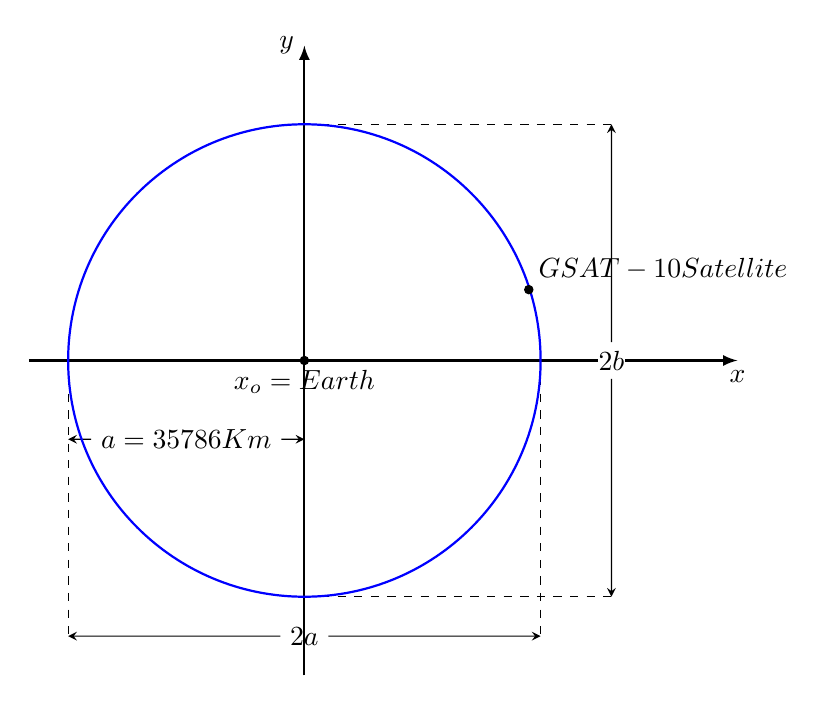
\begin{tikzpicture}

		% Axis
		\draw[-latex, thick] (3.5,0) -- (3.5,8) node[left] {$y$};
		\draw[-latex, thick] (0,4) -- (9,4) node[below] {$x$};

		% Lines
		\draw[dashed] (0.5,4) -- (0.5,0.5);
		\draw[dashed] (6.5,4) -- (6.5,0.5);
		%left key
		\draw[dashed] (3.5,1) -- (7.4,1);
		\draw[dashed] (3.5,7) -- (7.4,7);
		%% Labeled
		\midlinelabel{0.5,0.5}{6.5,0.5}{$2a$}
		\midlinelabel{0.5,3}{3.5,3}{$a = 35 786 Km$}
		%
		\midlinelabell{7.4,1}{7.4,7}{$2b$}

		% Ellipse
		\draw[blue, thick] (3.5,4) circle [x radius = 3, y radius = 3];

		% Points
		\draw[fill=black] (3.5,4) circle [radius=1.5pt] node[below] {$x_o = Earth$};
		\draw[fill=black] (6.35,4.9) circle [radius=1.5pt] node[above right] {$GSAT-10 Satellite$};
	\end{tikzpicture}

\end{document}
